\documentclass{article}
\usepackage{amsmath}
\usepackage{soul}
\usepackage{graphicx}
\graphicspath{ {./images/} }

\newcommand{\units}[1]{\texttt{#1}}
\newcommand{\biggbreak}{\\[1ex]}
\usepackage[margin=2cm]{geometry}


\begin{document}

\begin{figure}[h!]
  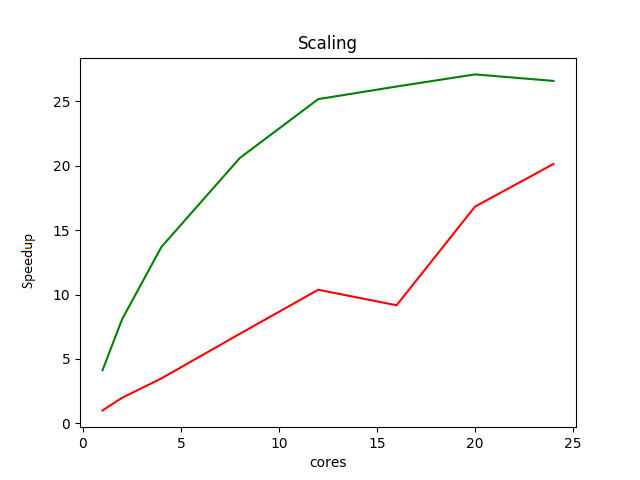
\includegraphics[scale=1]{scaling.png}
  \caption{Best case (red) - Many bodies throughout simulation (red) Difficult case - Start with many bodies that merge into 1 by thee end of simulation (green)}
  \label{fig:scaling}
\end{figure}

We see that both step-1 and step-3 converge as evident by parallel lines between both experiments for each method (step1, step3) trending towards 0 [Fig:\ref{fig:convergence}] From these lines we can calculate the approximate converge order for each step using their gradient. We see that step 1 has approximate convergence order $1.76$ and $1.84$; step 3 approximate convergence order $3.02$ and $2.86$. These approximate experimental converge orders match closely with the theoretical convergence values. Step 1, using Euler's method, has a theoretical convergence order $O(h^2)$ and step 3, using RK(2), $O(h^3)$. 


\begin{figure}[h!]
  \begin{center}
  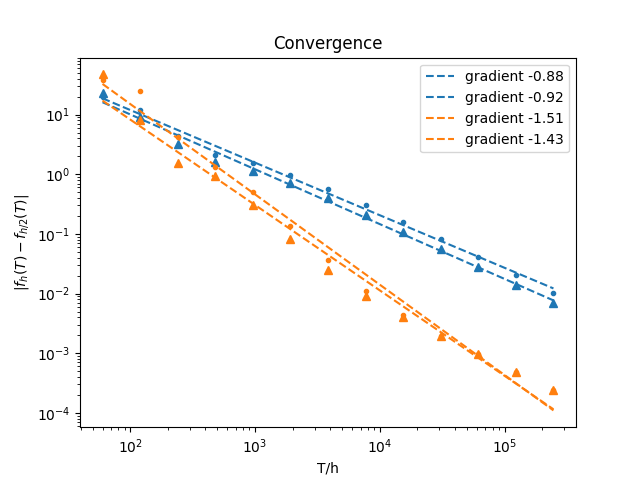
\includegraphics[scale=0.75]{convergence.png}
    \caption{step-1 (blue) step-3 (orange). Change in errors for a 2 body system under extreme condition (near collision).}
    \label{fig:convergence}
  \end{center}
  \end{figure}


 

\end{document}


